\chapter{Início Rápido}\label{cha:quickstart}

Este capítulo fornece instruções para se usar o XCSoar em provas normais de cross-country.  É separado em cenários simples para demostrar como usar as funções das teclas.  É assumido que as opções de configurações já foram ajustadas às preferências do usuário.

Estas instruções tem a intenção de fornecer um guia simples de passo a passo para voar as provas em vários níveis de complexidade mas não tem a finalidade de demonstrar todas as características do XCSoar.  Além do mais, o sistema pode ser usado em formas mais produtivas do que outras, como descrito aqui.



\section{Vôo local}\label{sec:local-flight}

Neste cenário, o piloto pretende voar localmente ou em uma prova de cross-country normal onde a navegação por waypoints pré-determinados não é necessária.

\subsection*{Antes da decolagem}
\begin{enumerate}
\item  Ligue o dispositivo.
\item  Abra a janela \button{Flight} e configure os bugs (insetos) e lastros necessários.  Ajuste a temperatura máxima prevista.  Feche a janela.
\item  Abra a janela  \button{Gerenciador de Tarefas} e crie uma nova prova teclando em \button{Nova Prova}.
\item  Selecione  ``Racing'' como tipo de prova.
\item  Uma vez criada a prova, mova o cursor para "Adicionar pilão" e tecle ENTER.  Selecione o waypoint da lista – o primeiro item é o item ‘casa’ e tecle SELEC.  
\item Selecione outro "Adicionar pilão", e entre o mesmo waypoint para ponto final.
\item  Agora a prova contém somente um ponto para casa.
\end{enumerate}

\subsection*{Em vôo}
\begin{enumerate}
\item  No momento propício, ajuste manualmente o valor de MacCready através do menu Calculadora ou através do variômetro.
\item  Mude o valor de bugs/lastro se necessário.
\item  A qualquer momento, a aeronave pode alcançar a casa quando a barra de diferença de altitude estiver verde e apontar para cima.
\item  Opcionalmente, ative  \button{MC Auto} quando estiver pronto para retornar para casa.  Se o modo MacCready estiver em “Planeio final” ou “Ambos”, o sistema irá indicar a velocidade ideal para retornar à casa.
\end{enumerate}

\subsection*{Após o pouso}
\begin{enumerate}
\item  A janela \button{Estado} mostrará o tempo total de vôo. 
\item  A janela de análise pode ser usada para analisar ou rever o vôo.
\item  O replay do registrador IGC pode ser usado para ver o vôo.
\item  Estas ações podem ser feitas após desligar o dispositivo e religa-lo novamente.
\end{enumerate}

\section{Prova FAI}\label{sec:fai-task}

Neste cenário, o piloto pretende voar em uma prova de triângulo FAI com um único setor de início e avanço automático de waypoint.

\subsection*{Antes da decolagem}
\begin{enumerate}
\item  Ligue o dispositivo.
\item  Abra a janela \button{Ajuste de voo} e configure os bugs (insetos) e lastros necessários.  Ajuste a temperatura máxima prevista.  Feche a janela.
\item  Abra a janela \button{Gerenciador de Tarefas} e crie uma nova prova teclando em 
\button{Nova prova}. Selecione o tipo de prova como “Triângulo FAI”.
\item  Uma vez criada a prova, mova o cursor para “adicionar pilão” e tecle ENTER.  Selecione o waypoint da lista – o primeiro item é o item ‘casa’ e tecle SELEC.  
\item  Mova o cursor para “Adicionar Pilão” novamente e tecle ENTER.  Selecione o waypoint da lista e tecle “SELEC”.  Irá adicionar o primeiro waypoint da prova.
\item  Repita o procedimento para o segundo waypoint.  Uma boa idéia para char o segundo pilão é filtrar a lista de waypoint pela direção (+120°) e a distância apropriada da borda do triângulo.  O filtro fará a referência ao primeiro waypoint do triângulo.
\item  Repita o último ponto necessário para o waypoint adicional.  O último waypoint é o waypoint final.
\item  A prova foi composta. Você deve declará-la e enviar a prova para um registrador conectado.  
\end{enumerate}

\subsection*{Em vôo}
\begin{enumerate}
\item  O waypoint atual irá avançar automaticamente enquanto o piloto voa através das zonas de observação.
\item  Depois que a prova é iniciada, a janela  \button{Estado} pode ser aberta para verificar a validação do start.  “Larg válida” deve estar como verdadeira.  O tempo de largada pode ser revisto e a altura da largada é salva e é mostrada a altura mínima para finalizar a prova de acordo com as regras.
\item  A qualquer momento, a seta negra do rastro irá apontar para o próximo waypoint.  A seta azul irá apontar na direção que o planador dever ir em cruzeiro.
\item  Se \button{Zoom Auto} estiver ativado, o mapa irá automaticamente fazer o zoom nos waypoints da prova.
\item  No momento propício, ajuste o MacCready pelo menu Calculadora ou pelo variômetro conectado; ou ativando   \button{MC Auto}.
Se o modo MacCready está ajustado para ‘Planeio Final’ ou ‘Ambos’, o sistema irá indicar a velocidade ideal para retornar para casa e o valor de MacCready será ajustado para a taxa mínima de subida na qual é benéfica para continuar a subida.
\item  Mude o bugs/lastro se necessário.
\item  Se necessário, consulte a janela  \button{Análise}. 
\item  Se necessário, consulte a janela  \button{Estado}.  Mostra a hora de início, tempo percorrido da prova, hora estimada de chegada, velocidade média a prova, etc.
\item  A qualquer momento, quando a barra de diferença de altitude estiver verde e apontando para cima, o planador pode terminar a prova.

\end{enumerate}

\subsection*{Após o pouso}
Descrito na seção ~\ref{sec:local-flight}.


\section{Prova AAT Task, Armar Manual}\label{sec:aat-task-manual}

Neste cenário, o piloto pretende voar uma prova de triângulo AAT e irá armar manualmente o sistema de avanço de waypoint.


\subsection*{Antes da decolagem.}
\begin{enumerate}
\item  Ligue o dispositivo.
\item  Abra a janela ajuste de vôo e configure os bugs (insetos) e lastros necessários.  Ajuste a temperatura máxima prevista.  Feche a janela.
\item Abra a janela do \button{Gerenciador de Tarefas}e crie uma nova prova teclando \button{Nova prova}. Selecione “AAT” como tipo de prova.
\item  Uma vez criada a prova, mova o cursor para “adicionar pilão” e tecle ENTER.  Selecione o waypoint da lista – o primeiro item é o item ‘casa’ e tecle SELEC.  
\item  A prova AAT necessita de entrada adicional do tipo e tamanho da zona de observação.  Ajuste os parâmetros do setor AAT para este waypoint e tecle ‘SELEC’.
\item  Repita estes últimos dois passos necessários para waypoints adicionais.  O último waypoint é o ponto de chegada.
\item  A prova AAT foi composta.  Abra a  \button{Propriedades} e ajuste o tempo de prova.
\item  O tempo estimado para completar a prova com ajustes diferentes de MacCready pode ser visto através da  \button{Calculadora}.  Ajuste o valor de MacCready e veja o que o XCSoar sugere com ajuste para o alcance AAT.
\end{enumerate}

\subsection*{Em vôo}
\begin{enumerate}
\item Quando o piloto está pronto para iniciar a prova, tecle o botão  \button{Armar Largada}. O waypoint atual avançará automaticamente somente uma vez, enquanto o piloto voa através do setor de início.  Após este momento, o gatilho de avanço é desarmado.
\item  Para que reinicie a prova, o piloto precisa reverter manualmente ao ponto de início novamente e apertar 
\button{Avançar Pilão} antes de voar através do setor de início novamente.
\item  Depois da prova iniciada a janela  \button{Estado} pode ser aberta para verificar se o início foi validado.  Se a hora do início é especificada, o start foi detectado e está legal conforme as regras da prova e especificado nas configurações, caso contrário será mostrado “INVALIDADO”.
\item  Durante o vôo, o tempo estimado para finalizar a prova com diferentes ajustes de MacCready pode ser explorado através da janela \button{Calculadora}.
  Uma vez tomada a decisão de estender ou reduzir o alcance AAT, pode ser feito manualmente manipulando \button{Pilões}. Isto permite ao piloto aumentar ou diminuir a distância da prova e estimar os resultados no tempo AAT. 

A figura abaixo mostra o curso ao redor dos pilões em um alcance ajustado para -100\%.
\begin{center}
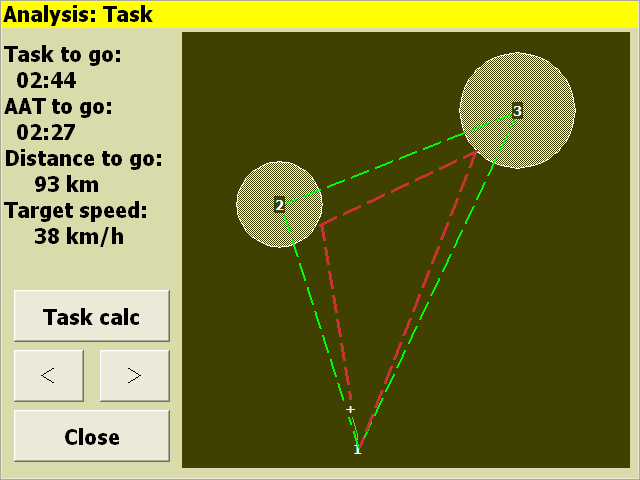
\includegraphics[angle=0,width=0.8\linewidth,keepaspectratio='true']{figures/aat-short.png}
\end{center}

A figura abaixo mostra o curso ao redor dos alvos em um alcance ajustado em 100\%.
\begin{center}
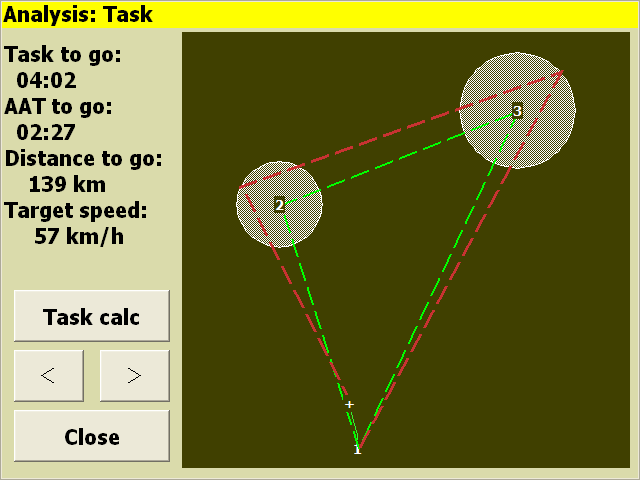
\includegraphics[angle=0,width=0.8\linewidth,keepaspectratio='true']{figures/aat-long.png}
\end{center}

\item  A todo momento, a seta preta irá apontar para o próximo pilão.  O pilão é localizado dentro do setor AAT com alcance especificado na janela  \button{Calc Prova}.  A seta azul irá apontar na direção que o planador deverá navegar em cruzeiro.

\item  Quando o piloto está se aproximando ou está dentro de um setor AAT e está pronto para avançar para o próximo waypoint, aperte  \button{Armar Pilão}.  O waypoint atual irá avançar automaticamente se o piloto estiver na zona de observação.  Após este ocorrido, o gatilho de avanço é desarmado.

\item Se o Autozoom estiver ativo, o mapa irá automaticamente mostrar os waypoints da prova.

\item  No momento propício, ajuste o MacCready pelo menu \button{Calc Prova} ou pelo variômetro conectado ou então ative \button{MC Auto}.
 Se o modo MacCready estiver em ‘Planeio final’ ou ‘Ambos, o sistema irá sugerir a velocidade ideal para retornar à casa e o valor de MacCready será ajustado para a taxa mínima de subida que é benéfica para continuar a subir.  
  
\item  Mude o bugs/lastro se necessário.
\item  Consulte \button{Análise}, se necessário. 
\item  Consulte a janela \button{Estado} se necessário.  Mostrará a hora de início, tempo gasto na prova, tempo estimado para chegada, velocidade média da prova, etc. 
\end{enumerate}

\subsection*{Após o pouso}
Descrito na seção ~\ref{sec:local-flight}.

% Agian in 6.1 
%\section{Task with alternate start sectors}
%
%In this scenario, the pilot intends to fly a task with 
%alternate start sectors and manually arm the waypoint advance system.
%
%\subsection*{Prior to takeoff}
%As described in Section~\ref{sec:fai-task}, except where noted below.
%\begin{enumerate}
%\item Open the `Task edit' dialogue, and set `Auto Advance' to `Arm start'.
%  Select the start waypoint, and press enter.  Set `Alternate Start
%  Points' to ON, and press `Edit start points'.  Press `clear' to
%  clear the list of existing start points if required.  Move the
%  cursor to a blank line or `add waypoint' line and press enter; then
%  select the waypoint and press enter.  Repeat for each alternate
%  start point.
%\end{enumerate}
%
%\subsection*{In-flight}
%As described in Section~\ref{sec:fai-task}, except where noted below.
%\begin{enumerate}
%\item 
%Prior to entering the start sector, when the pilot is ready to start
%the task, press the `Arm Advance' button.
%
%\item 
%In order to re-start from any start sector, the pilot needs to press
%the `Arm Advance' button again prior to flying through any of the
%start sectors again.
%\end{enumerate}

